\section{Absolute positioning}

\subsection{Triangulation}

Triangulation is an old method for positioning developed for use in land surveying. It is based around measuring the angles from visible landmarks to an assumed heading, usually either magnetic north or the facing of a robot. The original method was based around using a map and compass. The surveyor would then draw a line from the landmark such that it held the measured angle to magnetic north, this process will then be repeated several times. Once the process is complete, then the lines should intersect in a single point, or at least converge around a similar area. Any line that does not land in an area close to the intersection point can then be assumed to be a erroneous and discarded or redone. The convergence point or area can then be assumed to be the surveyors location.

\subsection{Trilateration}

Trilateration works by measuring the distance to a minimum of three beacons and finding the intersection point between the circles created. Each measurement will give a center point, the beacon position, and a radius, the distance measured. The position can then be extrapolated by calculating the intersection points of the circles using the readers preferred method.

\subsection{ToTAL algorithm}

The ToTal algorithm\footnote{\cite{VincentPierlot2001}} is a method for performing triangulation without the use of a map or compass, for use by a robot or similar device. The algorithm has certain benefits over previous work in that it has no requirement for which order the beacons are measured in, and it is resilient to mathematical outliers when the robot is not inside the triangle formed by the beacons. However it does have some prerequisites that must be fulfilled before it can work:

\begin{enumerate}
\item The absolute positions of the beacons must be known. 
\item The robot must know its own facing. This is necessary to get the orientation of the robot. 
\item The robot must have a counterclockwise rotating receiver for reading the beacons, in case the sensor is rotating clockwise then some of the formulas need to be inverted.
\end{enumerate}

The basic concepts of the algorithm are that it is possible to convert two known points (beacons) and an angle into a circle with a known size and center. Once that is done the problem has been converted to a simple trilateration problem, which is less computationally complex than previous forms of angular calculations. The algorithm in full is exhibited in figure \ref{fig:totalalgdrawing}\footnote{\cite{VincentPierlot2001}}.

\begin{figure}[H]
    \centering
    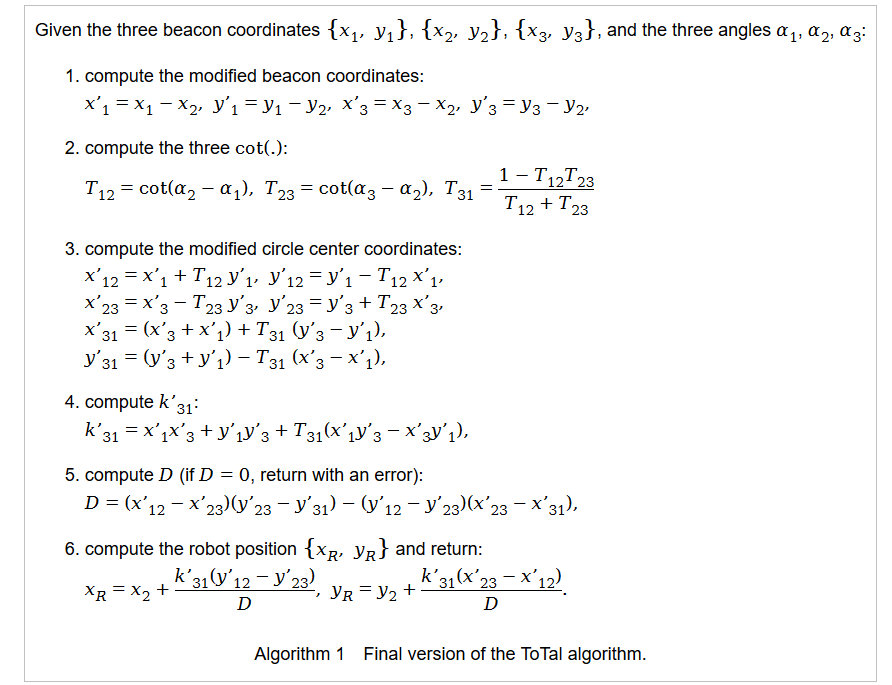
\includegraphics[width=0.7\linewidth]{positioning/positioning/ToTalAlgorithm}
    \caption{A snippet of the math making up the ToTAL algorithm.}
    \label{fig:totalalgdrawing}
\end{figure}
